% Options for packages loaded elsewhere
% Options for packages loaded elsewhere
\PassOptionsToPackage{unicode}{hyperref}
\PassOptionsToPackage{hyphens}{url}
\PassOptionsToPackage{dvipsnames,svgnames,x11names}{xcolor}
%
\documentclass[
  a4paper,
]{article}
\usepackage{xcolor}
\usepackage{amsmath,amssymb}
\setcounter{secnumdepth}{5}
\usepackage{iftex}
\ifPDFTeX
  \usepackage[T1]{fontenc}
  \usepackage[utf8]{inputenc}
  \usepackage{textcomp} % provide euro and other symbols
\else % if luatex or xetex
  \usepackage{unicode-math} % this also loads fontspec
  \defaultfontfeatures{Scale=MatchLowercase}
  \defaultfontfeatures[\rmfamily]{Ligatures=TeX,Scale=1}
\fi
\usepackage{lmodern}
\ifPDFTeX\else
  % xetex/luatex font selection
  \setmainfont[]{Latin Modern Roman}
  \setsansfont[]{Latin Modern Sans}
  \setmonofont[]{Latin Modern Mono}
\fi
% Use upquote if available, for straight quotes in verbatim environments
\IfFileExists{upquote.sty}{\usepackage{upquote}}{}
\IfFileExists{microtype.sty}{% use microtype if available
  \usepackage[]{microtype}
  \UseMicrotypeSet[protrusion]{basicmath} % disable protrusion for tt fonts
}{}
\makeatletter
\@ifundefined{KOMAClassName}{% if non-KOMA class
  \IfFileExists{parskip.sty}{%
    \usepackage{parskip}
  }{% else
    \setlength{\parindent}{0pt}
    \setlength{\parskip}{6pt plus 2pt minus 1pt}}
}{% if KOMA class
  \KOMAoptions{parskip=half}}
\makeatother
% Make \paragraph and \subparagraph free-standing
\makeatletter
\ifx\paragraph\undefined\else
  \let\oldparagraph\paragraph
  \renewcommand{\paragraph}{
    \@ifstar
      \xxxParagraphStar
      \xxxParagraphNoStar
  }
  \newcommand{\xxxParagraphStar}[1]{\oldparagraph*{#1}\mbox{}}
  \newcommand{\xxxParagraphNoStar}[1]{\oldparagraph{#1}\mbox{}}
\fi
\ifx\subparagraph\undefined\else
  \let\oldsubparagraph\subparagraph
  \renewcommand{\subparagraph}{
    \@ifstar
      \xxxSubParagraphStar
      \xxxSubParagraphNoStar
  }
  \newcommand{\xxxSubParagraphStar}[1]{\oldsubparagraph*{#1}\mbox{}}
  \newcommand{\xxxSubParagraphNoStar}[1]{\oldsubparagraph{#1}\mbox{}}
\fi
\makeatother


\usepackage{longtable,booktabs,array}
\usepackage{calc} % for calculating minipage widths
% Correct order of tables after \paragraph or \subparagraph
\usepackage{etoolbox}
\makeatletter
\patchcmd\longtable{\par}{\if@noskipsec\mbox{}\fi\par}{}{}
\makeatother
% Allow footnotes in longtable head/foot
\IfFileExists{footnotehyper.sty}{\usepackage{footnotehyper}}{\usepackage{footnote}}
\makesavenoteenv{longtable}
\usepackage{graphicx}
\makeatletter
\newsavebox\pandoc@box
\newcommand*\pandocbounded[1]{% scales image to fit in text height/width
  \sbox\pandoc@box{#1}%
  \Gscale@div\@tempa{\textheight}{\dimexpr\ht\pandoc@box+\dp\pandoc@box\relax}%
  \Gscale@div\@tempb{\linewidth}{\wd\pandoc@box}%
  \ifdim\@tempb\p@<\@tempa\p@\let\@tempa\@tempb\fi% select the smaller of both
  \ifdim\@tempa\p@<\p@\scalebox{\@tempa}{\usebox\pandoc@box}%
  \else\usebox{\pandoc@box}%
  \fi%
}
% Set default figure placement to htbp
\def\fps@figure{htbp}
\makeatother


% definitions for citeproc citations
\NewDocumentCommand\citeproctext{}{}
\NewDocumentCommand\citeproc{mm}{%
  \begingroup\def\citeproctext{#2}\cite{#1}\endgroup}
\makeatletter
 % allow citations to break across lines
 \let\@cite@ofmt\@firstofone
 % avoid brackets around text for \cite:
 \def\@biblabel#1{}
 \def\@cite#1#2{{#1\if@tempswa , #2\fi}}
\makeatother
\newlength{\cslhangindent}
\setlength{\cslhangindent}{1.5em}
\newlength{\csllabelwidth}
\setlength{\csllabelwidth}{3em}
\newenvironment{CSLReferences}[2] % #1 hanging-indent, #2 entry-spacing
 {\begin{list}{}{%
  \setlength{\itemindent}{0pt}
  \setlength{\leftmargin}{0pt}
  \setlength{\parsep}{0pt}
  % turn on hanging indent if param 1 is 1
  \ifodd #1
   \setlength{\leftmargin}{\cslhangindent}
   \setlength{\itemindent}{-1\cslhangindent}
  \fi
  % set entry spacing
  \setlength{\itemsep}{#2\baselineskip}}}
 {\end{list}}
\usepackage{calc}
\newcommand{\CSLBlock}[1]{\hfill\break\parbox[t]{\linewidth}{\strut\ignorespaces#1\strut}}
\newcommand{\CSLLeftMargin}[1]{\parbox[t]{\csllabelwidth}{\strut#1\strut}}
\newcommand{\CSLRightInline}[1]{\parbox[t]{\linewidth - \csllabelwidth}{\strut#1\strut}}
\newcommand{\CSLIndent}[1]{\hspace{\cslhangindent}#1}



\setlength{\emergencystretch}{3em} % prevent overfull lines

\providecommand{\tightlist}{%
  \setlength{\itemsep}{0pt}\setlength{\parskip}{0pt}}



 


\usepackage{booktabs}
\usepackage{longtable}
\usepackage{array}
\usepackage{multirow}
\usepackage{wrapfig}
\usepackage{float}
\usepackage{colortbl}
\usepackage{pdflscape}
\usepackage{tabu}
\usepackage{threeparttable}
\usepackage{threeparttablex}
\usepackage[normalem]{ulem}
\usepackage{makecell}
\usepackage{xcolor}
\usepackage{fancyhdr}
\pagestyle{fancy}
\fancyhf{}
\fancyhead[L]{\nouppercase{\leftmark}}
\fancyhead[R]{\thepage}
\renewcommand{\headrulewidth}{0.4pt}
\usepackage[english,mt]{ethidsc}
\studentA{Marc Jerónimo Pérez y Ropero}
\ethidA{13-938-311}
\emailA{marcpe@ethz.ch}
\supervision{Prof. Dr. Emmanuel Frossard \\ Dr. Frank Liebisch}
\declaration
\infopage
\makeatletter
\@ifpackageloaded{caption}{}{\usepackage{caption}}
\AtBeginDocument{%
\ifdefined\contentsname
  \renewcommand*\contentsname{Table of contents}
\else
  \newcommand\contentsname{Table of contents}
\fi
\ifdefined\listfigurename
  \renewcommand*\listfigurename{List of Figures}
\else
  \newcommand\listfigurename{List of Figures}
\fi
\ifdefined\listtablename
  \renewcommand*\listtablename{List of Tables}
\else
  \newcommand\listtablename{List of Tables}
\fi
\ifdefined\figurename
  \renewcommand*\figurename{Figure}
\else
  \newcommand\figurename{Figure}
\fi
\ifdefined\tablename
  \renewcommand*\tablename{Table}
\else
  \newcommand\tablename{Table}
\fi
}
\@ifpackageloaded{float}{}{\usepackage{float}}
\floatstyle{ruled}
\@ifundefined{c@chapter}{\newfloat{codelisting}{h}{lop}}{\newfloat{codelisting}{h}{lop}[chapter]}
\floatname{codelisting}{Listing}
\newcommand*\listoflistings{\listof{codelisting}{List of Listings}}
\makeatother
\makeatletter
\makeatother
\makeatletter
\@ifpackageloaded{caption}{}{\usepackage{caption}}
\@ifpackageloaded{subcaption}{}{\usepackage{subcaption}}
\makeatother
\usepackage{bookmark}
\IfFileExists{xurl.sty}{\usepackage{xurl}}{} % add URL line breaks if available
\urlstyle{same}
\hypersetup{
  pdftitle={Master Thesis},
  colorlinks=true,
  linkcolor={blue},
  filecolor={Maroon},
  citecolor={Blue},
  urlcolor={Blue},
  pdfcreator={LaTeX via pandoc}}


\title{Master Thesis}
\author{Marc Pérez}
\date{}
\begin{document}
\maketitle
\begin{abstract}
Hier kommt das Abstract
\end{abstract}

\maketitle
\tableofcontents

\listoffigures
\listoftables

\section{Abstract}\label{abstract}

\section{Introduction}\label{introduction}

\subsection{The Complexity of
Phosphorus}\label{the-complexity-of-phosphorus}

Phosphorus (P) is an essential macronutrient for all known life, forming
a critical part of DNA and energy-transfer molecules. In soils---where
organic, mineral, and aqueous phases interface---its behavior is
complex. In the presence of oxygen, P exists almost exclusively as
orthophosphate (\(PO_4^{3-}\)) and its protonated forms (\(HPO_4^{2-}\)
or \(H_2PO_4^{-}\)), depending on the soil pH. These dissolved phosphate
species are highly reactive; they are subject to adsorption onto the
surfaces of clays and oxides and can precipitate with cations like
calcium, iron, and aluminum to form minerals with low solubility.
Consequently, while the total amount of P in a soil can be large, only a
small fraction is in the soil solution at any given moment, posing a
central challenge for agriculture. The efficacy of P fertilization is
often low due to these rapid immobilization processes, and P lost from
agricultural fields can become an environmental pollutant, disturbing
P-limited aquatic ecosystems.

\textbf{Soil organic matter (SOM) adds another layer of complexity to
these interactions.} Organic acids released during the decomposition of
SOM can compete with phosphate for the same adsorption sites on mineral
surfaces, which can increase P concentrations in the soil solution.
Furthermore, humic substances can form stable complexes with cations
like Al³⁺ and Fe³⁺, preventing them from precipitating phosphate and
thereby enhancing its availability. The efficacy of P fertilization is
often low due to these rapid and competing immobilization processes, and
P lost from agricultural fields can become an environmental pollutant,
disturbing P-limited aquatic ecosystems.

\subsection{From Static Measurements to Dynamic
Understanding}\label{from-static-measurements-to-dynamic-understanding}

To manage this challenge, traditional soil testing methods (e.g.,
Olsen-P, AAE10, CO₂-water) were developed to quantify the \textbf{size
of the readily available P pool}. This static measurement is often
referred to as the \textbf{``capacity factor''}. While these tests are
invaluable for basic fertility assessment, they do not capture the
dynamic nature of P supply. A crucial missing piece of information is
the rate at which P is replenished into the soil solution from the solid
phase after being taken up by plant roots. This replenishment rate, or
\textbf{``kinetic factor''}, is vital for sustaining crop growth,
especially during periods of high demand.

The importance of these dynamics is not a new concept. As early as 1982,
\textbf{Flossmann and Richter} argued that characterizing the kinetics
of P release was essential for refining fertilizer recommendations
beyond what static tests alone could offer. Modern research has
reinforced this view, showing that fertilization strategies based solely
on maintaining a critical soil test P (STP) concentration can be
inefficient. In Switzerland, this has led to the accumulation of
``legacy P'' in many agricultural soils, and understanding the release
kinetics of this legacy P is key to both improving nutrient efficiency
and protecting water quality. Furthermore, critical STP levels are not
constant; they are influenced by pedoclimatic factors like soil texture
and temperature, making a ``one-size-fits-all'' approach to
fertilization suboptimal.

\subsection{Objectives and Research
Questions}\label{objectives-and-research-questions}

An ideal set of parameters for P management should meet several
criteria. The parameters should correlate strongly with P export and P
balance in a steady-state system. They must also respond to fertilizer
inputs and, most importantly, capture the diffusive, kinetic nature of P
supply to plant roots.

This thesis hypothesizes that \textbf{kinetic parameters describing P
desorption, derived from a simple laboratory extraction, can serve as
effective predictors for agronomic outcomes.} Using soils from the
long-term STYCS experiment in Switzerland, this study employs a modified
version of the Flossmann \& Richter kinetic test to derive the
desorption rate (\(k\)) and the desorbable P pool (\(P_{desorb}\)). The
performance of these new kinetic parameters will be compared against
standard STP methods (\(P_{CO_2}\) and \(P_{AAE10}\)) by addressing the
following research questions:

\begin{enumerate}
\def\labelenumi{\arabic{enumi}.}
\tightlist
\item
  Is the P desorption kinetic method replicable and effective for the
  soils from the STYCS trial?
\item
  How do the kinetic coefficients, \(k\) and \(P^S\), correlate with key
  soil properties (organic carbon, clay content, pH)?
\item
  How well do the standard STP methods (\(P_{CO_2}\) \& \(P_{AAE10}\))
  predict crop yield, P export, and P balance?
\item
  Can the kinetic parameters, \(k\) and \(P^S\), improve the prediction
  of these agronomic outcomes compared to the standard static tests?
\end{enumerate}

\section{Materials and Methods}\label{sec-materials-and-methods}

\subsection{The Long-Term Phosphorus Fertilization
Experiment}\label{sec-the-long-term-phosphorus-fertilization-experiment}

The soil samples for this thesis originate from a set of six long-term
field trials in Switzerland, established by Agroscope between 1989 and
1992. The primary objective of these experiments was to validate and
re-evaluate Swiss phosphorus (P) fertilization guidelines by assessing
long-term crop yield responses to varying P inputs across different
pedoclimatic conditions. A detailed description of the experimental
design and site characteristics can be found in (Hirte et al., 2021)

The experiment was set up as a \textbf{completely randomized block
design} with four field replications at each site. The core of the
experiment consists of six fixed-plot treatments representing different
P fertilization levels, which were applied annually as superphosphate
before tillage and sowing. These levels were based on percentages of the
officially recommended P inputs: 0\% (Zero), 33\% (Deficit), 67\%
(Reduced), 100\% (Norm), 133\% (Elevated), and 167\% (Surplus).

\subsection{Experimental Sites}\label{sec-experimental-sites}

The six experimental sites are located in the main crop-growing regions
of Switzerland: \textbf{Rümlang-Altwi (ALT)}, \textbf{Cadenazzo (CAD)},
\textbf{Ellighausen (ELL)}, \textbf{Grabs (GRA)}, \textbf{Oensingen
(OEN)}, and \textbf{Zurich-Reckenholz (REC)}. The key soil properties
are summarized below.

\begin{longtable}[]{@{}
  >{\raggedright\arraybackslash}p{(\linewidth - 10\tabcolsep) * \real{0.0704}}
  >{\raggedright\arraybackslash}p{(\linewidth - 10\tabcolsep) * \real{0.3099}}
  >{\raggedleft\arraybackslash}p{(\linewidth - 10\tabcolsep) * \real{0.1268}}
  >{\raggedleft\arraybackslash}p{(\linewidth - 10\tabcolsep) * \real{0.1268}}
  >{\raggedleft\arraybackslash}p{(\linewidth - 10\tabcolsep) * \real{0.2394}}
  >{\raggedleft\arraybackslash}p{(\linewidth - 10\tabcolsep) * \real{0.1268}}@{}}

\caption{\label{tbl-sites-corrected}Soil characteristics of the six
long-term experimental sites. Data adapted from Hirte et al.~(2021).}

\tabularnewline

\toprule\noalign{}
\begin{minipage}[b]{\linewidth}\raggedright
Site
\end{minipage} & \begin{minipage}[b]{\linewidth}\raggedright
Soil Type (WRB)
\end{minipage} & \begin{minipage}[b]{\linewidth}\raggedleft
Clay (\%)
\end{minipage} & \begin{minipage}[b]{\linewidth}\raggedleft
Sand (\%)
\end{minipage} & \begin{minipage}[b]{\linewidth}\raggedleft
Organic C (g/kg)
\end{minipage} & \begin{minipage}[b]{\linewidth}\raggedleft
pH (H2O)
\end{minipage} \\
\midrule\noalign{}
\endhead
\bottomrule\noalign{}
\endlastfoot
ALT & Calcaric Cambisol & 22 & 48 & 21 & 7.9 \\
CAD & Eutric Fluvisol & 8 & 40 & 14 & 6.3 \\
ELL & Eutric Cambisol & 33 & 31 & 23 & 6.6 \\
GRA & Calcaric Fluvisol & 17 & 34 & 16 & 8.3 \\
OEN & Gleyic-calc. Cambisol & 37 & 32 & 24 & 7.1 \\
REC & Eutric Gleysol & 39 & 25 & 27 & 7.4 \\

\end{longtable}

\textsubscript{Source:
\href{https://Andrapodon.github.io/Master-Thesis-P-kinetics/index.qmd.html}{Article
Notebook}}

Soil samples for this thesis were collected on {[}Your Sampling Date{]}
from the topsoil layer (0-20 cm). {[}Add any further specific details
about your sampling strategy here{]}.

\begin{center}\rule{0.5\linewidth}{0.5pt}\end{center}

\subsection{Phosphorus Desorption
Kinetics}\label{sec-phosphorus-desorption-kinetics}

The analysis of phosphorus (P) desorption kinetics was based on the
principles of sequential extraction established by Flossmann and Richter
(1982). The original method is described below, followed by the specific
protocol adapted for this study.

\subsubsection{Original Method of Flossmann and Richter (1982)
\{\#sec-original-method-of-flossmann-and-richter-(1982\}}\label{original-method-of-flossmann-and-richter-1982-sec-original-method-of-flossmann-and-richter-1982}

The foundational method aims to characterize the P replenishment
capacity of the soil. The procedure is as follows:

\begin{enumerate}
\def\labelenumi{\arabic{enumi}.}
\tightlist
\item
  \textbf{Removal of Soluble P}: 17.5 g of air-dried soil is shaken with
  350 ml of deionized water for one hour at 25 ± 1°C. The suspension is
  centrifuged and the supernatant is decanted to remove the readily
  soluble P fraction. This first extract is referred to as:

  \begin{itemize}
  \tightlist
  \item
    \textbf{Solution A}: Contains easily soluble P, which is discarded.
  \end{itemize}
\item
  \textbf{Kinetic Extraction}: The remaining soil pellet is resuspended
  with another 350 ml of deionized water. Subsamples of the suspension
  are taken at specific time intervals, yielding the following extracts
  for kinetic analysis:

  \begin{itemize}
  \tightlist
  \item
    \textbf{Solution B}: Subsample taken after \textbf{10 minutes}.
  \item
    \textbf{Solution C}: Subsample taken after \textbf{30 minutes}.
  \item
    \textbf{Solution D}: Subsample taken after \textbf{120 minutes}.
  \end{itemize}
\item
  \textbf{Analysis}: The P concentration in Solutions B, C, and D is
  determined colorimetrically using the molybdenum blue method according
  to Murphy and Riley (1962).
\end{enumerate}

\subsubsection{Adapted Kinetic Protocol for This
Study}\label{sec-adapted-kinetic-protocol-for-this-study}

For this thesis, the original method was modified to capture the
desorption process with a higher temporal resolution and using a
different soil-to-solution ratio.

\begin{enumerate}
\def\labelenumi{\arabic{enumi}.}
\item
  \textbf{Soil Suspension}: 10 g of air-dried soil was suspended in 200
  ml of deionized water. Unlike the original protocol, a pre-washing
  step to remove soluble P was not performed, meaning the measured
  desorption includes both the release of readily soluble P and the
  subsequent replenishment from the solid phase.
\item
  \textbf{Kinetic Extraction}: The suspension was shaken continuously,
  and subsamples were taken at eight time points to generate a detailed
  kinetic curve. The resulting extracts were:

  \begin{itemize}
  \tightlist
  \item
    \textbf{Extract 1}: Subsample taken after \textbf{2 minutes}.
  \item
    \textbf{Extract 2}: Subsample taken after \textbf{4 minutes}.
  \item
    \textbf{Extract 3}: Subsample taken after \textbf{10 minutes}.
  \item
    \textbf{Extract 4}: Subsample taken after \textbf{15 minutes}.
  \item
    \textbf{Extract 5}: Subsample taken after \textbf{20 minutes}.
  \item
    \textbf{Extract 6}: Subsample taken after \textbf{30 minutes}.
  \item
    \textbf{Extract 7}: Subsample taken after \textbf{45 minutes}.
  \item
    \textbf{Extract 8}: Subsample taken after \textbf{60 minutes}.
  \end{itemize}
\item
  \textbf{Analysis}: Each subsample was immediately filtered. The
  concentration of orthophosphate in the filtered extracts was
  determined colorimetrically using the \textbf{malachite green method}.
\end{enumerate}

\begin{center}\rule{0.5\linewidth}{0.5pt}\end{center}

\begin{figure}[H]

{\centering \pandocbounded{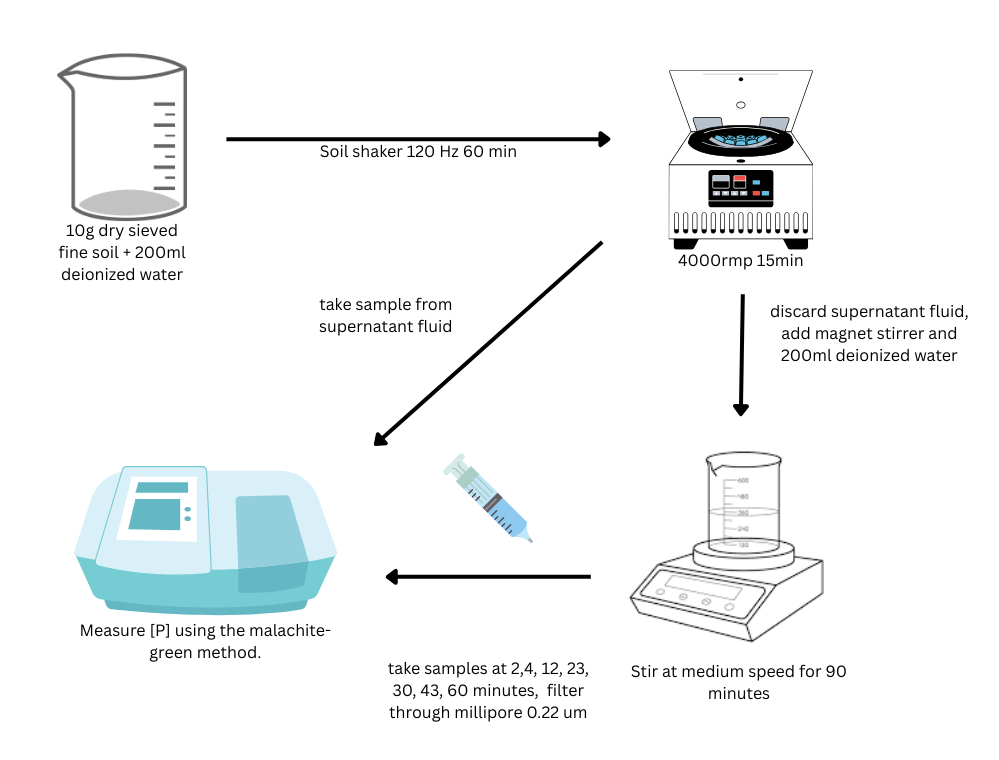
\includegraphics[keepaspectratio]{./experiment-flow.png}}

}

\caption{Flow-chart of the adapted Kinetik-experiment after Flossmann \&
Richter.}

\end{figure}%

\subsection{Statistical Analysis}\label{sec-statistical-analysis}

The statistical workflow involved two main stages: 1) estimating the P
desorption kinetic parameters from the laboratory data, and 2) using
these parameters to model the agronomic outcomes from the long-term
field experiment.

\subsubsection{Modeling of Desorption
Kinetics}\label{sec-modeling-of-desorption-kinetics}

To derive the kinetic parameters, a non-linear mixed-effects model
(\texttt{nlme}) was implemented. This approach was chosen to
simultaneously estimate the rate constant (\(k\)) and the maximum
desorbable P (\(P_{desorb}\)) directly from the time-series data for
each soil sample. The model was fitted to the exact solution of the
first-order rate equation:

\[ P(t) = P_{desorb} \times (1 - e^{-k \times t'}) \]

Where \(P(t)\) is the P concentration at time \(t\), and \(t'\) is an
adjusted time (\(t_\text{min} + 3\) min) to account for rapid initial P
dissolution. The overall means for \(P_{desorb}\) and \(k\) were modeled
as \textbf{fixed effects}, while sample-specific deviations for both
parameters were modeled as \textbf{random effects} to capture the unique
characteristics of each soil sample.

\subsubsection{Modeling of Agronomic
Responses}\label{sec-modeling-of-agronomic-responses}

The estimated kinetic parameters were merged with the agronomic and soil
chemistry dataset from the years 2017-2022. A series of linear
mixed-effects models were then constructed to evaluate the predictive
power of these parameters.

\paragraph{Variables Used in the
Models}\label{sec-variables-used-in-the-models}

The response and predictor variables used in the linear mixed-effects
models are defined in the table below.

\begin{longtable}[]{@{}
  >{\raggedright\arraybackslash}p{(\linewidth - 6\tabcolsep) * \real{0.0855}}
  >{\raggedright\arraybackslash}p{(\linewidth - 6\tabcolsep) * \real{0.1447}}
  >{\raggedright\arraybackslash}p{(\linewidth - 6\tabcolsep) * \real{0.0658}}
  >{\raggedright\arraybackslash}p{(\linewidth - 6\tabcolsep) * \real{0.7039}}@{}}

\caption{\label{tbl-variables}Description of variables used in the
agronomic models.}

\tabularnewline

\toprule\noalign{}
\begin{minipage}[b]{\linewidth}\raggedright
Abbreviation
\end{minipage} & \begin{minipage}[b]{\linewidth}\raggedright
Full.Name
\end{minipage} & \begin{minipage}[b]{\linewidth}\raggedright
Role
\end{minipage} & \begin{minipage}[b]{\linewidth}\raggedright
Description
\end{minipage} \\
\midrule\noalign{}
\endhead
\bottomrule\noalign{}
\endlastfoot
\(Y_{rel}\) & Relative Yield & Response & Plot yield normalized by the
national mean yield for that year and crop. \\
\(Y_{norm}\) & Normalized Yield & Response & Plot yield normalized by
the site-specific median yield of the highest P treatment for that year
and crop. \\
\(P_{up}\) & P Uptake & Response & Total P removed by the harvested crop
biomass over a growing season (kg P ha⁻¹). \\
\(P_{bal}\) & P Balance & Response & Net P budget, calculated as P
inputs (fertilizer) minus P outputs (uptake) (kg P ha⁻¹). \\
\(k\) & Rate Constant & Predictor & First-order rate constant of P
desorption, representing the speed of P release (min⁻¹). \\
\(P_{desorb}\) & Desorbable P & Predictor & Maximum desorbable P,
representing the size of the readily available P pool (mg P L⁻¹). \\
\(J_0\) & Initial P Flux & Predictor & Product of \(k\) and
\(P_{desorb}\), representing the initial flux of P from the soil. \\
\(P_{CO2}\) & Water-Soluble P & Predictor & Plant-available P measured
by the CO₂-saturated water extraction method (mg P kg⁻¹). \\
\(P_{AAE10}\) & Chelate-Extractable P & Predictor & Plant-available P
measured by the ammonium-acetate-EDTA extraction method (mg P kg⁻¹). \\

\end{longtable}

\textsubscript{Source:
\href{https://Andrapodon.github.io/Master-Thesis-P-kinetics/index.qmd.html}{Article
Notebook}}

\paragraph{Linear Mixed-Effects Model
Structure}\label{sec-linear-mixed-effects-model-structure}

Linear mixed-effects models (\texttt{lmer}) were used to test the
relationships between the predictor variables and each of the three
response variables. The structure of these models was designed to
account for the nested nature of the long-term experiment. A general
form of the model is:

\emph{Response Variable \textasciitilde{} Fixed Effects + (1 \textbar{}
Random Effects)}

\begin{itemize}
\tightlist
\item
  \textbf{Fixed Effects}: These represent the main explanatory variables
  of interest whose effects we wanted to quantify. The fixed effects
  included the kinetic parameters (\(k\), \(P_{desorb}\), \(J_0\)) and
  the standard soil P tests (\(P_w\), \(P_{AAE10}\)), along with their
  interactions.
\item
  \textbf{Random Effects}: These were included to control for
  non-independence among observations. By including
  \texttt{(1\ \textbar{}\ Site)}, \texttt{(1\ \textbar{}\ Year)}, and
  \texttt{(1\ \textbar{}\ Crop)} as random intercepts, the model
  accounts for baseline differences in the response variable that are
  attributable to the specific location, growing season, or crop type,
  allowing for a more accurate estimation of the fixed effects.
\end{itemize}

To identify the most informative and parsimonious model, a systematic
feature selection process was conducted using the \texttt{mlr3} machine
learning framework. This involved training and evaluating different
combinations of predictor variables using nested cross-validation to
ensure the robustness of the final selected model.

All statistical analyses were performed in the R environment, utilizing
the \texttt{nlme} package for kinetic modeling and the \texttt{lme4},
\texttt{lmerTest}, and \texttt{mlr3} packages for the final agronomic
modeling and feature selection.

\section{Results}\label{results}

\textsubscript{Source:
\href{https://Andrapodon.github.io/Master-Thesis-P-kinetics/index.qmd.html}{Article
Notebook}}

The results of this study are presented in two main parts. First, the
development and validation of the phosphorus (P) desorption kinetic
model are detailed, justifying the final modeling approach. Second, the
descriptive trends of both agronomic outcomes and soil P parameters in
response to long-term fertilization and site differences are explored
visually. Finally, the predictive power of the kinetic and standard P
parameters is formally evaluated using linear mixed-effects models.

\subsection{Establishment of the P-Desorption Kinetic
Model}\label{establishment-of-the-p-desorption-kinetic-model}

The primary goal was to derive two key parameters for each soil sample:
the desorbable P pool (\(P_{desorb}\)) and the rate constant (\(k\)).
The analysis proceeded in two stages: an initial test of a linearized
model, followed by the implementation of a more robust non-linear model.

\subsubsection{Initial Approach: Failure of the Linearized
Model}\label{initial-approach-failure-of-the-linearized-model}

Following the conceptual framework of Flossmann and Richter (1982), the
first-order kinetic equation was linearized. A core assumption of this
model is that the linear relationship must pass through the origin. To
test this, linear models were fitted to the transformed data for each
sample individually. The results revealed a systematic failure of this
assumption, as the estimated intercepts for the majority of samples were
highly significantly different from zero (p \textless{} 0.05). This
consistent statistical deviation indicated that the linearized approach
was not a valid representation of the data. The visual evidence in
Figure~\ref{fig-linearized-model} supports this conclusion.

\phantomsection\label{cell-fig-linearized-model}
\begin{figure}[H]

\centering{

\pandocbounded{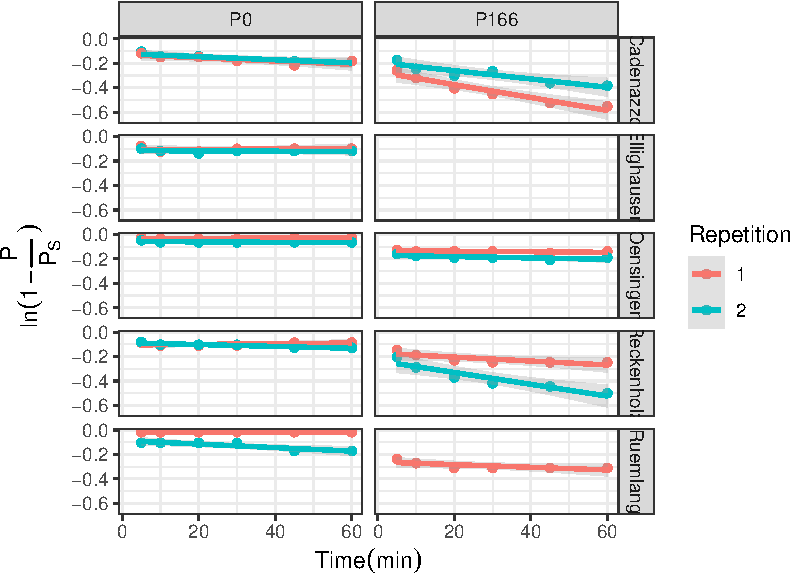
\includegraphics[keepaspectratio]{index_files/figure-pdf/fig-linearized-model-1.pdf}}

}

\caption{\label{fig-linearized-model}Test of the linearized first-order
kinetic model. The plot visually supports the statistical finding that
many intercepts are not zero.}

\end{figure}%

\textsubscript{Source:
\href{https://Andrapodon.github.io/Master-Thesis-P-kinetics/index.qmd.html}{Article
Notebook}}

\subsubsection{Final Approach: Successful Non-Linear
Model}\label{final-approach-successful-non-linear-model}

Given the statistical failure of the linearized model, a direct
non-linear modeling approach was adopted to estimate both \(P_{desorb}\)
and \(k\) simultaneously from the untransformed data. This approach does
not rely on the assumption of a zero intercept and proved to be far more
successful, accurately capturing the curvilinear shape of the desorption
data for nearly all samples (fig-nonlinear-model). The final parameters
were extracted from a non-linear mixed-effects model (\texttt{nlme}) to
account for the hierarchical data structure. \textbf{These final
\texttt{nlme}-derived coefficients were used for all subsequent
analyses.}

\phantomsection\label{cell-fig-nonlinear-model}
\begin{figure}[H]

\centering{

\pandocbounded{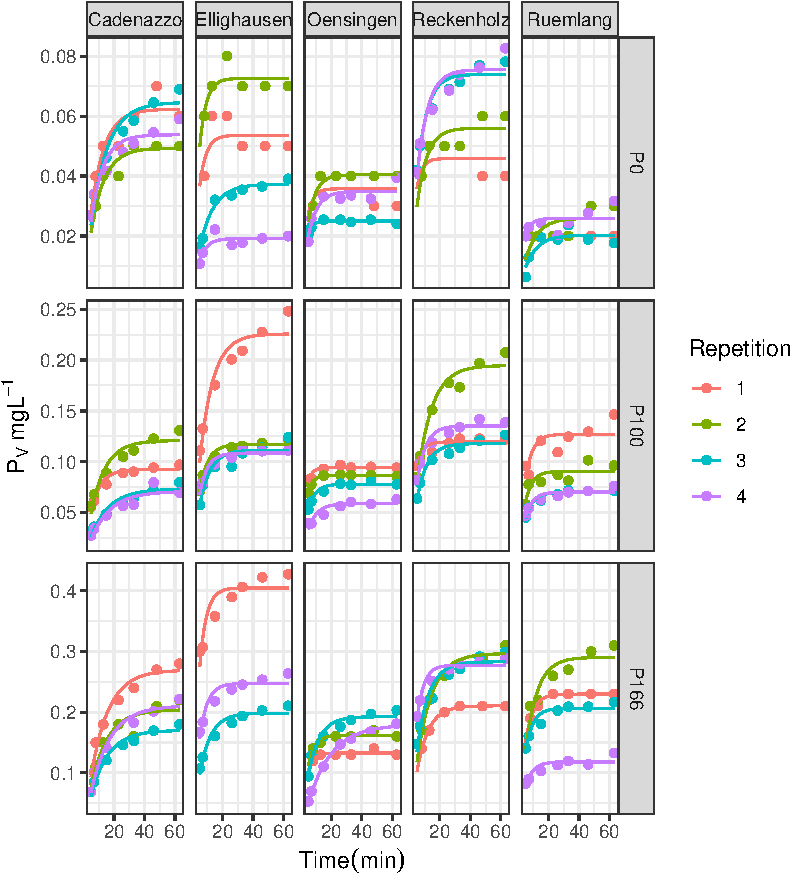
\includegraphics[keepaspectratio]{index_files/figure-pdf/fig-nonlinear-model-1.pdf}}

}

\caption{\label{fig-nonlinear-model}Non-linear first-order kinetic model
fits for P desorption over time. Points represent measured data and
solid lines represent the fitted model for each replicate.}

\end{figure}%

\textsubscript{Source:
\href{https://Andrapodon.github.io/Master-Thesis-P-kinetics/index.qmd.html}{Article
Notebook}}

\subsection{Comparison with Isotopic Exchange Kinetics (IEK)
\{\#sec-comparison-with-isotopic-exchange-kinetics-(iek\}}\label{comparison-with-isotopic-exchange-kinetics-iek-sec-comparison-with-isotopic-exchange-kinetics-iek}

To validate the newly derived kinetic parameters against an established
benchmark, the capacity (\(P_{desorb}\)) and kinetic (\(k\)) parameters
were compared to data from Isotopic Exchange Kinetics (IEK) studies
previously conducted on the same long-term trial sites by Demaria et
al.~(2013). This comparison aims to determine if the simpler,
non-equilibrium desorption method used in this thesis captures similar
aspects of soil P dynamics as the more complex, equilibrium-based IEK
method.

The size of the desorbable P pool (\(P_{desorb}\)) was compared against
the long-term isotopically exchangeable P pool measured after 7 days
(\(E_{exp\_10080}\)). The desorption rate constant (\(k\)) was compared
against the IEK kinetic parameter measured after 24 hours
(\(n_{1440}\)). Spearman's rank correlation was used to robustly test
for monotonic trends between the different methods.

\begin{figure}

\begin{minipage}{0.50\linewidth}

\centering{

\pandocbounded{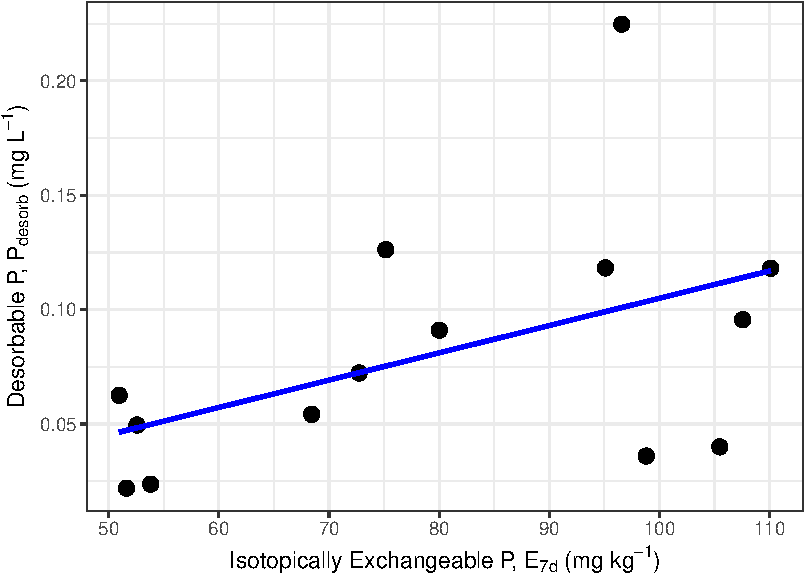
\includegraphics[keepaspectratio]{index_files/figure-pdf/fig-iek-comparison-1.pdf}}

}

\subcaption{\label{fig-iek-comparison-1}Capacity: \(P_{\text{desorb}}\)
vs \(E_{\text{7d}}\)}

\end{minipage}%
%
\begin{minipage}{0.50\linewidth}

\centering{

\pandocbounded{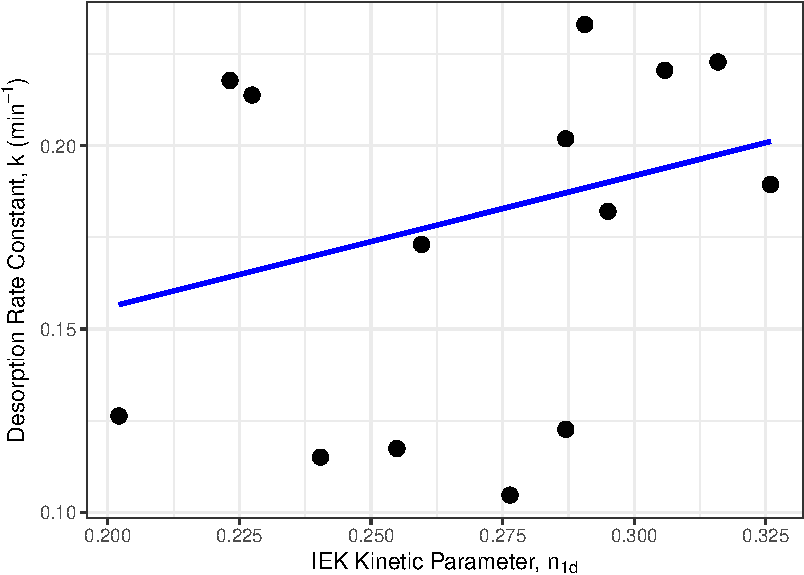
\includegraphics[keepaspectratio]{index_files/figure-pdf/fig-iek-comparison-2.pdf}}

}

\subcaption{\label{fig-iek-comparison-2}Kinetics: k vs
\(n_{\text{1d}}\)}

\end{minipage}%

\caption{\label{fig-iek-comparison}Correlation between
desorption-derived kinetic parameters and IEK-derived parameters. (A)
Capacity parameters: Desorbable P (\(P_{\text{desorb}}\))
vs.~Isotopically Exchangeable P (\(E_{\text{7d}}\)). (B) Kinetic
parameters: Rate Constant (\(k\)) vs.~IEK kinetic parameter
(\(n_{\text{1d}}\)).}

\end{figure}%

The analysis revealed a statistically significant, moderate positive
correlation between the capacity parameters, \(P_{desorb}\) and
\(E_{exp\_10080}\) (fig-iek-comparison). The Spearman's rank correlation
coefficient was 0.4 with a p-value of \textless{} 0.001.

Similarly, a statistically significant, moderate positive correlation
was found between the kinetic parameters, \(k\) and \(n_{1440}\)
(fig-iek-comparison). The Spearman's rank correlation coefficient was
0.36 with a p-value of \textless{} 0.001.

These results indicate that the simpler, non-equilibrium desorption
method used in this study successfully captures both the capacity and
intensity aspects of soil P lability, providing results that are
consistent with the more complex, equilibrium-based IEK method reported
by Demaria et al.~(2013).

\subsection{Effects of Fertilization on Agronomic and Soil
Parameters}\label{sec-effects-of-fertilization-on-agronomic-and-soil-parameters}

Having established a robust method to determine the kinetic parameters,
the next step was to explore the effects of the long-term P
fertilization treatments on both the agronomic outcomes and the soil P
test parameters.

\subsubsection{Agronomic Responses to P
Fertilization}\label{sec-agronomic-responses-to-p-fertilization}

The long-term application of different P fertilization levels had a
pronounced impact on the primary agronomic outcomes, including two
different metrics for yield, P Uptake (\(P_{up}\)), and P Balance
(\(P_{bal}\)), though the response varied considerably between sites
(Figure~\ref{fig-agronomic-responses}).

\phantomsection\label{cell-fig-agronomic-responses}
\begin{figure}[H]

\centering{

\pandocbounded{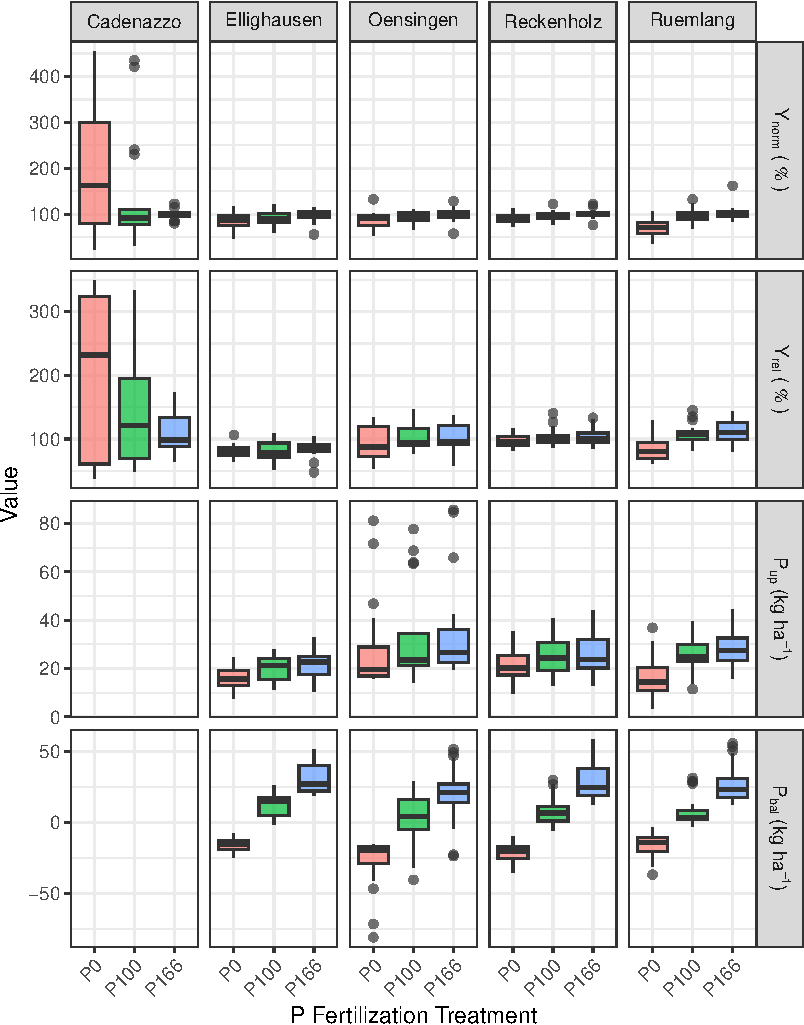
\includegraphics[keepaspectratio]{index_files/figure-pdf/fig-agronomic-responses-1.pdf}}

}

\caption{\label{fig-agronomic-responses}Agronomic response variables
across six P fertilization treatments and six experimental sites. Data
from 2017-2022.}

\end{figure}%

\textsubscript{Source:
\href{https://Andrapodon.github.io/Master-Thesis-P-kinetics/index.qmd.html}{Article
Notebook}}

\textbf{Yield Metrics (}\(Y_{norm}\) and \(Y_{rel}\)): Both yield
metrics showed a generally positive response to P fertilization. The
site-normalized yield (\(Y_{norm}\)) shows the response relative to the
site's potential for that year, with most yields plateauing around the
Norm (100\%) treatment. The national-normalized yield (\(Y_{rel}\))
provides a broader context, showing how yields at each site compare to
the national average.

\textbf{P Uptake (}\(P_{up}\)): P uptake by crops followed a similar
trend to yield, increasing with fertilization, often continuing to
increase at the highest fertilization levels, suggesting luxury
consumption.

\textbf{P Balance (}\(P_{bal}\)): The P balance showed a strong, linear
relationship with fertilization. The Zero and Deficit treatments
resulted in a negative balance (mining soil P), while the Elevated and
Surplus treatments led to a significant P surplus.

\subsubsection{Soil P Parameters as a Function of P
Fertilization}\label{sec-soil-p-parameters-as-a-function-of-p-fertilization}

The different soil P test parameters, including the standard STP methods
and the newly derived kinetic parameters, all responded to the long-term
fertilization treatments (Figure~\ref{fig-soil-parameters}).

\phantomsection\label{cell-fig-soil-parameters}
\begin{figure}[H]

\centering{

\pandocbounded{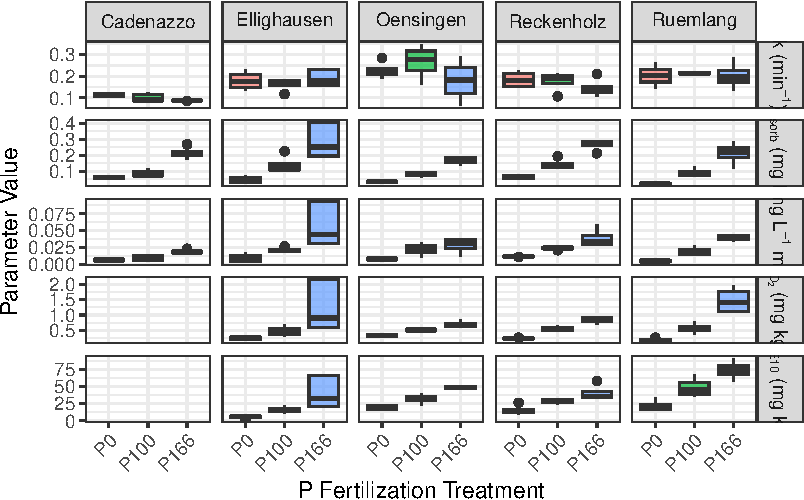
\includegraphics[keepaspectratio]{index_files/figure-pdf/fig-soil-parameters-1.pdf}}

}

\caption{\label{fig-soil-parameters}Soil P parameters across six P
fertilization treatments and six experimental sites.}

\end{figure}%

\textsubscript{Source:
\href{https://Andrapodon.github.io/Master-Thesis-P-kinetics/index.qmd.html}{Article
Notebook}}

\textbf{Standard STPs (}\(P_{CO_2}\) and \(P_{AAE10}\)): Both standard
soil P tests showed a clear and consistent increase with rising P
fertilization levels across all sites, confirming their sensitivity to
management.

\textbf{Kinetic Parameters (}\(k\), \(P_{desorb}\), and \(J_0\)): *
\textbf{Desorbable P (}\(P_{desorb}\)): This parameter behaved very
similarly to the standard STPs, increasing steadily with P fertilization
and confirming its role as a ``capacity'' indicator. * \textbf{Rate
Constant (}\(k\)): The rate constant showed a more complex pattern, with
no strong, consistent trend with fertilization. This suggests that while
fertilization increases the \emph{amount} of available P, it may not
change the intrinsic \emph{release rate}. * \textbf{Initial P Flux
(}\(J_0\)): As the product of \(P_{desorb}\) and \(k\), this parameter
integrates both capacity and intensity. It showed a strong positive
response to fertilization, driven primarily by the increase in
\(P_{desorb}\).

These initial observations suggest that the kinetic parameters,
particularly the rate constant \(k\), may provide unique information
about the soil's P dynamics not captured by static tests alone. The next
section will use formal statistical models to test these relationships.

\subsection{Predicting P Parameters from Soil
Properties}\label{sec-p-params-soil-props}

To understand the underlying drivers of the standard and kinetic P
parameters, a series of linear mixed-effects models were fitted. Each
model predicted one of the P parameters based on the core soil
properties: organic carbon (\(C_{org}\)), clay content, silt content,
pH, and amorphous Al/Fe oxides. The models included random effects for
\texttt{Site}, \texttt{Year}, and \texttt{Block}. The results are
summarized in Table~\ref{tbl-soil-prop-models}.

\begin{longtable}[]{@{}llllll@{}}

\caption{\label{tbl-soil-prop-models}Results of linear mixed-effects
models predicting P parameters from intrinsic soil properties.
Significance codes: `\emph{\textbf{' p \textless{} 0.001, '}' p
\textless{} 0.01, '}' p \textless{} 0.05.}

\tabularnewline

\toprule\noalign{}
Model & \(P_{desorb}\) & \(k\) & \(J_0\) & \(P_{CO_2}\) &
\(P_{AAE10}\) \\
\midrule\noalign{}
\endhead
\bottomrule\noalign{}
\endlastfoot
Intercept & 21.444*** & 0.454 & 21.189*** & 14.014** & 23.126** \\
Ald & -8.706*** & -0.072 & -8.631* & -4.417 & -9.473* \\
Fed & -1.068*** & 0.005 & -1.084 & -0.845* & -0.606 \\
Clay & -0.006 & -0.016** & -0.085 & 0.015 & -0.029 \\
\(C_{org}\) & 0.612* & 0.137** & 1.250* & 0.269 & 1.454*** \\
pH & -0.018 & -0.021 & -0.092 & 0.124 & 0.012 \\
Silt & -0.000 & 0.004 & 0.008 & -0.015 & -0.049* \\
\(R^2_m\) & 0.393 & 0.212 & 0.368 & 0.362 & 0.494 \\
\(R^2_c\) & 0.996 & 0.915 & 0.993 & 0.995 & 0.997 \\

\end{longtable}

\textsubscript{Source:
\href{https://Andrapodon.github.io/Master-Thesis-P-kinetics/index.qmd.html}{Article
Notebook}}

The analysis in Table~\ref{tbl-soil-prop-models} reveals that the
capacity-based P pools and the kinetic rate constant are controlled by
different sets of soil properties. Both amorphous aluminum (\(Al_{ox}\))
and iron (\(Fe_{ox}\)) oxides had a highly significant negative effect
on the \textbf{Desorbable P pool (}\(P_{desorb}\)), suggesting they bind
P strongly. In contrast, \textbf{Organic Carbon (}\(C_{org}\)) had a
significant positive effect on all capacity measures, especially
\texttt{\$P\_\{AAE10\}\$}. The \textbf{Rate Constant (}\(k\)) was not
significantly driven by the oxides, but showed a significant positive
relationship with \texttt{\$C\_\{org\}\$} and a negative relationship
with \texttt{Clay} content, indicating that the speed of P release is
governed by different mechanisms than the total pool size.

\subsection{Predictive Modeling of Agronomic
Outcomes}\label{sec-agronomic-modeling}

To formally evaluate and compare the predictive power of the standard
STP methods against the newly derived kinetic parameters, a series of
linear mixed-effects models (\texttt{lmer}) were fitted for each of the
primary agronomic response variables.

\subsubsection{\texorpdfstring{Predicting Site-Normalized Yield
(\(Y_{norm}\))}{Predicting Site-Normalized Yield (Y\_\{norm\})}}\label{sec-ynorm}

The models predicting the site-normalized yield are summarized in
Table~\ref{tbl-ynorm-models}. For this metric, the standard STP methods
proved to be the most effective predictors.

\begin{longtable}[]{@{}
  >{\raggedright\arraybackslash}p{(\linewidth - 8\tabcolsep) * \real{0.1931}}
  >{\raggedright\arraybackslash}p{(\linewidth - 8\tabcolsep) * \real{0.1724}}
  >{\raggedright\arraybackslash}p{(\linewidth - 8\tabcolsep) * \real{0.1793}}
  >{\raggedright\arraybackslash}p{(\linewidth - 8\tabcolsep) * \real{0.2414}}
  >{\raggedright\arraybackslash}p{(\linewidth - 8\tabcolsep) * \real{0.2138}}@{}}

\caption{\label{tbl-ynorm-models}Results of linear mixed-effects models
predicting Site-Normalized Yield (\(Y_{norm}\)).}

\tabularnewline

\toprule\noalign{}
\begin{minipage}[b]{\linewidth}\raggedright
Model
\end{minipage} & \begin{minipage}[b]{\linewidth}\raggedright
\(Y_{norm} \sim P_{CO_2}\)
\end{minipage} & \begin{minipage}[b]{\linewidth}\raggedright
\(Y_{norm} \sim P_{AAE10}\)
\end{minipage} & \begin{minipage}[b]{\linewidth}\raggedright
\(Y_{norm} \sim P_{CO_2}*P_{AAE10}\)
\end{minipage} & \begin{minipage}[b]{\linewidth}\raggedright
\(Y_{norm} \sim k * P_{desorb}\)
\end{minipage} \\
\midrule\noalign{}
\endhead
\bottomrule\noalign{}
\endlastfoot
Intercept & 1.059*** & 0.532*** & 1.096*** & 0.980 \\
\(k\) & & & & 2.262 \\
\(J_0\) & & & & 0.931 \\
\(log(P_{desorb})\) & & & & -0.063 \\
\(log(P_{AAE10})\) & & 0.120*** & -0.006 & \\
\(log(P_{CO_2})\) & 0.162*** & & 0.137 & \\
\(P_{CO_2} \times P_{AAE10}\) & & & 0.016 & \\
\(R^2_m\) & 0.218 & 0.198 & 0.220 & 0.014 \\
\(R^2_c\) & 0.358 & 0.474 & 0.365 & 0.360 \\

\end{longtable}

\textsubscript{Source:
\href{https://Andrapodon.github.io/Master-Thesis-P-kinetics/index.qmd.html}{Article
Notebook}}

As shown in Table~\ref{tbl-ynorm-models}, both \texttt{\$P\_\{CO\_2\}\$}
and \texttt{\$P\_\{AAE10\}\$} were highly significant predictors of
site-normalized yield, with the model containing
\texttt{\$P\_\{CO\_2\}\$} explaining the most variance (Marginal R² =
0.218). In contrast, the kinetic parameters showed no significant
predictive power for \texttt{\$Y\_\{norm\}\$}.

\subsubsection{\texorpdfstring{Predicting National-Normalized Yield
(\(Y_{rel}\))}{Predicting National-Normalized Yield (Y\_\{rel\})}}\label{sec-yrel}

When predicting the yield normalized to the national average, the
kinetic parameters demonstrated a much stronger performance, as
summarized in Table~\ref{tbl-yrel-models}.

\begin{longtable}[]{@{}
  >{\raggedright\arraybackslash}p{(\linewidth - 8\tabcolsep) * \real{0.1986}}
  >{\raggedright\arraybackslash}p{(\linewidth - 8\tabcolsep) * \real{0.1702}}
  >{\raggedright\arraybackslash}p{(\linewidth - 8\tabcolsep) * \real{0.1773}}
  >{\raggedright\arraybackslash}p{(\linewidth - 8\tabcolsep) * \real{0.2411}}
  >{\raggedright\arraybackslash}p{(\linewidth - 8\tabcolsep) * \real{0.2128}}@{}}

\caption{\label{tbl-yrel-models}Results of linear mixed-effects models
predicting National-Normalized Yield (\(Y_{rel}\)).}

\tabularnewline

\toprule\noalign{}
\begin{minipage}[b]{\linewidth}\raggedright
Model
\end{minipage} & \begin{minipage}[b]{\linewidth}\raggedright
\(Y_{rel} \sim P_{CO_2}\)
\end{minipage} & \begin{minipage}[b]{\linewidth}\raggedright
\(Y_{rel} \sim P_{AAE10}\)
\end{minipage} & \begin{minipage}[b]{\linewidth}\raggedright
\(Y_{rel} \sim P_{CO_2}*P_{AAE10}\)
\end{minipage} & \begin{minipage}[b]{\linewidth}\raggedright
\(Y_{rel} \sim k * P_{desorb}\)
\end{minipage} \\
\midrule\noalign{}
\endhead
\bottomrule\noalign{}
\endlastfoot
Intercept & 104.862*** & 75.343*** & 130.274*** & 56.375 \\
\(k\) & & & & 377.498** \\
\(J_0\) & & & & 171.507** \\
\(log(P_{desorb})\) & & & & -27.486* \\
\(log(P_{AAE10})\) & & 7.111** & -6.537 & \\
\(log(P_{CO_2})\) & 8.853** & & 23.091 & \\
\(P_{CO_2} \times P_{AAE10}\) & & & -3.110 & \\
\(R^2_m\) & 0.074 & 0.063 & 0.078 & 0.022 \\
\(R^2_c\) & 0.569 & 0.537 & 0.596 & 0.439 \\

\end{longtable}

\textsubscript{Source:
\href{https://Andrapodon.github.io/Master-Thesis-P-kinetics/index.qmd.html}{Article
Notebook}}

As seen in Table~\ref{tbl-yrel-models}, while the standard STP methods
were also significant predictors, the kinetic model revealed a
significant positive effect of the \textbf{Rate Constant (}\(k\)) and
its interaction with \texttt{\$P\_\{desorb\}\$} (\texttt{\$J\_0\$}).
This suggests that the speed of P release is a more important factor
when comparing yields across the broader environmental gradient
represented by the national average.

\subsubsection{\texorpdfstring{Predicting P-Export
(\(P_{up}\))}{Predicting P-Export (P\_\{up\})}}\label{sec-pexport}

For predicting P-Export, the standard STP methods performed very well,
with the kinetic model showing comparable, albeit non-significant,
performance, as shown in Table~\ref{tbl-pexport-models}.

\begin{longtable}[]{@{}
  >{\raggedright\arraybackslash}p{(\linewidth - 8\tabcolsep) * \real{0.2044}}
  >{\raggedright\arraybackslash}p{(\linewidth - 8\tabcolsep) * \real{0.1679}}
  >{\raggedright\arraybackslash}p{(\linewidth - 8\tabcolsep) * \real{0.1752}}
  >{\raggedright\arraybackslash}p{(\linewidth - 8\tabcolsep) * \real{0.2409}}
  >{\raggedright\arraybackslash}p{(\linewidth - 8\tabcolsep) * \real{0.2117}}@{}}

\caption{\label{tbl-pexport-models}Results of linear mixed-effects
models predicting P-Export (\(P_{up}\)).}

\tabularnewline

\toprule\noalign{}
\begin{minipage}[b]{\linewidth}\raggedright
Model
\end{minipage} & \begin{minipage}[b]{\linewidth}\raggedright
\(P_{up} \sim P_{CO_2}\)
\end{minipage} & \begin{minipage}[b]{\linewidth}\raggedright
\(P_{up} \sim P_{AAE10}\)
\end{minipage} & \begin{minipage}[b]{\linewidth}\raggedright
\(P_{up} \sim P_{CO_2}*P_{AAE10}\)
\end{minipage} & \begin{minipage}[b]{\linewidth}\raggedright
\(P_{up} \sim k * P_{desorb}\)
\end{minipage} \\
\midrule\noalign{}
\endhead
\bottomrule\noalign{}
\endlastfoot
Intercept & 27.522*** & 8.090 & 30.632* & 29.599*** \\
\(k\) & & & & 22.622 \\
\(J_0\) & & & & 11.928 \\
\(log(P_{desorb})\) & & & & 1.954 \\
\(log(P_{AAE10})\) & & 4.824*** & -0.805 & \\
\(log(P_{CO_2})\) & 5.177*** & & 8.069 & \\
\(P_{CO_2} \times P_{AAE10}\) & & & -0.814 & \\
\(R^2_m\) & 0.064 & 0.073 & 0.065 & 0.064 \\
\(R^2_c\) & 0.625 & 0.603 & 0.623 & 0.648 \\

\end{longtable}

\textsubscript{Source:
\href{https://Andrapodon.github.io/Master-Thesis-P-kinetics/index.qmd.html}{Article
Notebook}}

The results in Table~\ref{tbl-pexport-models} show that both
\texttt{\$P\_\{CO\_2\}\$} and \texttt{\$P\_\{AAE10\}\$} were highly
significant predictors, explaining around 6-7\% of the variance
(marginal R²). This suggests that the size of the available P pool is a
robust indicator of the amount of P a crop will take up.

\subsubsection{\texorpdfstring{Predicting P-Balance
(\(P_{bal}\))}{Predicting P-Balance (P\_\{bal\})}}\label{sec-pbalance}

The most striking result was found when predicting the P-Balance,
summarized in Table~\ref{tbl-pbalance-models}. The standard STP methods
showed no significant ability to predict the P-Balance, whereas the
kinetic model was a powerful predictor.

\begin{longtable}[]{@{}
  >{\raggedright\arraybackslash}p{(\linewidth - 8\tabcolsep) * \real{0.1986}}
  >{\raggedright\arraybackslash}p{(\linewidth - 8\tabcolsep) * \real{0.1702}}
  >{\raggedright\arraybackslash}p{(\linewidth - 8\tabcolsep) * \real{0.1773}}
  >{\raggedright\arraybackslash}p{(\linewidth - 8\tabcolsep) * \real{0.2411}}
  >{\raggedright\arraybackslash}p{(\linewidth - 8\tabcolsep) * \real{0.2128}}@{}}

\caption{\label{tbl-pbalance-models}Results of linear mixed-effects
models predicting P-Balance (\(P_{bal}\)).}

\tabularnewline

\toprule\noalign{}
\begin{minipage}[b]{\linewidth}\raggedright
Model
\end{minipage} & \begin{minipage}[b]{\linewidth}\raggedright
\(P_{bal} \sim P_{CO_2}\)
\end{minipage} & \begin{minipage}[b]{\linewidth}\raggedright
\(P_{bal} \sim P_{AAE10}\)
\end{minipage} & \begin{minipage}[b]{\linewidth}\raggedright
\(P_{bal} \sim P_{CO_2}*P_{AAE10}\)
\end{minipage} & \begin{minipage}[b]{\linewidth}\raggedright
\(P_{bal} \sim k * P_{desorb}\)
\end{minipage} \\
\midrule\noalign{}
\endhead
\bottomrule\noalign{}
\endlastfoot
Intercept & 4.441 & 7.691 & 3.649 & 43.833*** \\
\(k\) & & & & 84.993 \\
\(J_0\) & & & & 33.029 \\
\(log(P_{desorb})\) & & & & 16.947*** \\
\(log(P_{AAE10})\) & & -0.794 & 0.187 & \\
\(log(P_{CO_2})\) & -0.928 & & -2.442 & \\
\(P_{CO_2} \times P_{AAE10}\) & & & 0.462 & \\
\(R^2_m\) & 0.001 & 0.001 & 0.001 & 0.572 \\
\(R^2_c\) & 0.810 & 0.807 & 0.811 & 0.744 \\

\end{longtable}

\textsubscript{Source:
\href{https://Andrapodon.github.io/Master-Thesis-P-kinetics/index.qmd.html}{Article
Notebook}}

As detailed in Table~\ref{tbl-pbalance-models}, the kinetic model
explained \textbf{57\% of the variance} in P-Balance (marginal R² =
0.572), with the \textbf{Desorbable P pool (}\(P_{desorb}\)) being the
dominant, highly significant predictor. This indicates that the
\texttt{\$P\_\{desorb\}\$} parameter from the kinetic experiment is a
vastly superior measure of the soil's P budget compared to standard STP
tests.

\section{Discussion}\label{discussion}

\section{Conclusion}\label{conclusion}

\section{Acknowledgments}\label{acknowledgments}

\section{Legal Disclosure}\label{legal-disclosure}

\section{References}\label{references}

\phantomsection\label{refs}
\begin{CSLReferences}{1}{0}
\bibitem[\citeproctext]{ref-hirte_yield_2021}
Hirte, J., Richner, W., Orth, B., Liebisch, F., \& Flisch, R. (2021).
Yield response to soil test phosphorus in switzerland: Pedoclimatic
drivers of critical concentrations for optimal crop yields using
multilevel modelling. \emph{Science of The Total Environment},
\emph{755}, 143453.
\url{https://doi.org/10.1016/j.scitotenv.2020.143453}

\end{CSLReferences}

\section{Appendix}\label{appendix}

\section{Supplements}\label{supplements}




\end{document}
